%
% File ACL2016.tex
%
\documentclass[11pt]{article}
\usepackage{fss2017seminar}
\usepackage{times}
\usepackage{latexsym}
\usepackage{graphicx}
\usepackage{amsmath,amssymb}
\usepackage{dsfont}
\graphicspath{ {img/} }

\aclfinalcopy % Uncomment this line for the final submission

% To expand the titlebox for more authors, uncomment
% below and set accordingly.
% \addtolength\titlebox{.5in}    

\newcommand\BibTeX{B{\sc ib}\TeX}


\title{Seminar: Generating Narrative Paragraph for Photo Stream }

% Author information can be set in various styles:
% For several authors from the same institution:
% \author{Author 1 \and ... \and Author n \\
%         Address line \\ ... \\ Address line}
% if the names do not fit well on one line use
%         Author 1 \\ {\bf Author 2} \\ ... \\ {\bf Author n} \\
% For authors from different institutions:
% \author{Author 1 \\ Address line \\  ... \\ Address line
%         \And  ... \And
%         Author n \\ Address line \\ ... \\ Address line}
% To start a seperate ``row'' of authors use \AND, as in
% \author{Author 1 \\ Address line \\  ... \\ Address line
%         \AND
%         Author 2 \\ Address line \\ ... \\ Address line \And
%         Author 3 \\ Address line \\ ... \\ Address line}
% If the title and author information does not fit in the area allocated,
% place \setlength\titlebox{<new height>} right after
% at the top, where <new height> can be something larger than 2.25in
\author{Chen Zongqi\\
	    Matriculation Number 1564832\\
	    University of Mannheim, Germany\\
	    {\tt zchen@mail.uni-mannheim.de}}

\date{}

\begin{document}

\maketitle

\begin{abstract}
When machine learning techniques develop rapidly in image captioning, other extension relevant areas appeal to many researchers doing further study. Among them generating story from sequential photo stream becomes quite interesting and challenging task. Compared with single image captioning, this task needs to handle with two mainly problems facing to researchers, large visual variance in sequence and long-term language coherence among multiple sentences. Till now those two critical questions are solved by different approaches. In this paper, we mainly focus on one of them, generating story from sequential photos stream via Bidirectional Attention Recurrent Neural Network method, and discus several relevant approaches from first paper to state-of-the-art.   
\end{abstract}

\section{Introduction}
With computing ability rapidly developing and new theory proposing, there are more and more intersection researches between computer vision area and natural language processing area occurring. This paper will focus on one specified topic from them, which is generating narrative paragraph for photo stream.  	

The basic task for this topic is that given sequential photos as input and return a story to describe as output. The core problems which need to be solved are how to generate corresponding sentence and how to organize sentences as human-level story. The previous question is based on the related field Image Captioning, such as generator with deep recurrent structure \cite{vinyals2014neural}, deep visual-semantic alignments  \cite{Karpathy:2017:DVA:3069214.3069250}. However the different between this topic with image captioning is that image captioning mainly focus on individual image and this topic needs to handle with sequential photos. It would be more challenged that computer not only needs to understand the content of images but also need to find their inner relation.   

This paper would introduce three approaches, Bidirectional Attention Recurrent Neural Network \cite{liu2017let}, Coherence Recurrent Convolutional Network \cite{NIPS2015_5776} and Generating Narrative Paragraph by Adversarial Training \cite{show-reward-tell-automatic-generation-narrative-paragraph-photo-stream-adversarial-training}. Meanwhile we want to introduce some basic terminologies which could be beneficial for understanding in background part, such as basic network structures and some language evaluation methods. Furthermore this paper would introduce main-stream datasets special for this field including some information about scale, content and generation strategy. Finally, we would compare their difference and common characteristics and discuss which parts could improve our evaluation and how could they work in last two parts Evaluation and Discussion. 

\section{Background}
In machine learning and natural language processing area, there are many high frequency terminologies appearing in almost every relevant paper and article. Here we list some significant terms mentioned in this paper having briefly explanation including different networks and retrieval methods.

{\bf Convolutional Neural Network} CNN is first implemented for application in 1998 by Yann LeCun \cite{lecun1998gradient} which applied for digit recognition experiment. CNN is developed from Neural Network \cite{hornik1989multilayer} which includes input layer, hidden layer and output layer. The basic CNN hidden layers contains convolutional layers, pooling layers, fully connected layers and normalization layers. The reason why CNN could develop so rapidly is that researchers start to use GPU to improve calculation efficiency \cite{steinkraus2005using}. Later some famous CNN networks are invited, such as AlexNet \cite{NIPS2012_4824}, GoogleNet \cite{szegedy2015going}, VGGNet \cite{Simonyan14c} and ResNet \cite{he2016deep}.

{\bf Recurrent Neural Network} RNN is another neural network variant, which connects each unit in a cycle way. One of the successful network Long short-term memory is invited to use as a block for developing a larger RNN network \cite{hochreiter1997long}. The basic components include cell, input gate, output gate and forget gate. In particularly, the concept of cell is very important for LSTM, which means memory. Due to RNN has many variants, here we list two of them such as bidirectional recurrent neural networks \cite{schuster1997bidirectional} and deep bidirectional recurrent neural networks \cite{graves2013speech}. RNN has huge success in natural language processing because of its special recurrent component. 

{\bf Generative Adversarial Networks } GANs are quite special neural network variant which contains game theory to train two neural networks \cite{goodfellow2014generative}. The basic idea is that two models, generative model an discriminative model, play a two-player game and leaning from each game result. GANs become more and more popular in deep learning area based on its powerful ability in handling with complex tasks.

{\bf BLEU} Bilingual evaluation understudy (BLEU) is quick,
inexpensive, and language-independent,
that correlates highly with human evaluation,
and that has little marginal cost per
run \cite{papineni2002bleu}. BLEU is a popular evaluation score for machine translation quality since 2002. BLEU has approximate human judgement at a corpus-level, whereas it has bad performance sometimes on sentence-level. See formula \ref{eq:BLUE} below :
\begin{equation}
\begin{aligned}
Pn &= \frac{\sum\sum Countclip(n-gram)}{\sum \sum Count(n-gram)} \\
BLEU &= BP \cdot \exp \left(\sum_{n=1}^{N} w_n \log p_n\right), \\
\end{aligned}
\label{eq:BLUE}
\end{equation}
where $Pn$ is the whole corpus modified precision score, $N$ is the length, $w_n$ is positive weights adding up to 1 and $BP$ is the brevity penalty function \ref{eq:bp} see below:
\begin{equation}
BP=\begin{cases}
               1, & \text{if} c > r\\
               e^{(1-r/c)}, & \text{otherwise}\\
            \end{cases}
\label{eq:bp}
\end{equation}
where $r$ is test corpus effective reference length and $c$ is the total length of the candidate translation corpus. 

{\bf METEOR} Metric for Evaluation of Translation with Explicit ORdering (METEOR)  is based on a generalized concept of
uni-gram matching between the machine produced
translation and human-produced
reference translations \cite{banerjee2005meteor}. Compared with BLEU, METEOR consider both precision and recall value on whole corpus. And METEOR has better performance in both corpus-level and sentence-level. Here is the basic formula \ref{eq:METEOR}:
\begin{equation}
\begin{aligned}
Fmean &= \frac{10PR}{R+9P} \\
Pen &= \gamma \left(\frac{ch}{m}\right)^{\theta} \\
METEOR &= (1-Pen) \cdot Fmean, \\
\end{aligned}
\label{eq:METEOR}
\end{equation}
where $P$ is precision value, $R$ is recall value, $ch$ is the number of chunks, $\gamma$ and $\theta$ are tuned
to maximize correlation with human judgements.


{\bf CIDEr} Consensus-based Image Description Evaluation (CIDEr) a novel paradigm for evaluating image descriptions that uses human consensus \cite{vedantam2015cider}. CIDEr treats each sentence as document using its tf-idf vector and compute caption with generative caption by cosine similarity. See equation \ref{eq:g} below:
\begin{equation}
\begin{aligned}
g(s_{ij}) = \frac{h_{k}(s_{ij})}{\sum h_{l} (s_{ij})} \log\left(\frac{|I|}{\sum\min(1,\sum_{q}h_{k}(s_{pq}))}\right),  
\end{aligned}
\label{eq:g}
\end{equation}
where $h_{k}(s_{ij})$ means the number of
times an n-gram $w_{k}$ occurs in a reference sentence $s_{ij}$, $|I|$ is  the set of all images in the dataset and $g(s_{ij})$  is tf-idf weighting for each n-gram $w_{k}$. From equation \ref{eq:g} we can find that the left part is actually to compute term frequency and right part $\log$ is to calculate idf. Finally, we can use $g$ as tf-idf weight to compute generative sentence and reference sentence cosine similarity.

If candidate sentence and reference sentence are more similar in vector space then their cosine similarity value is larger. See the formula below:
\begin{equation}
\begin{aligned}
CIDEr_{n}(c_{i},S_{i}) = \frac{1}{m} \sum_{j} \frac{g^{n}(c_{i}) \cdot g^{n}(s_{ij}) }{ |g^{n}(c_{i})| |g^{n}(s_{ij})|},
\end{aligned}
\label{eq:CIDEr}
\end{equation}
where $g^{n}(c_i)$is a vector formed by $g(c_i)$ corresponding to
all n-grams of length $n$ and $|g^{n}(c_i)|$ is the magnitude of the vector $g^n(c_i)$; $g^n(s_{ij})$ as well.

Finally we combine them from n-grams of varying lengths for the following equation \ref{eq:CIDE} as below:
\begin{equation}
\begin{aligned}
CIDEr(c_{i},S_{i}) = \sum_{n=1}^{N} w_n CIDEr_{n}(c_i,S_i),
\end{aligned}
\label{eq:CIDE}
\end{equation}
where uniform weights $w_n = \frac{1}{N} $work the best.


		
		
		
\section{Approach}
In this part, we mainly introduce our topic model Bidirectional Attentional Recurrent Neural Networks, and then briefly explain two related but important models, Coherence Recurrent Convolutional Network \cite{NIPS2015_5776} and Generating Narrative Paragraph by Adversarial Training \cite{show-reward-tell-automatic-generation-narrative-paragraph-photo-stream-adversarial-training}. Particularly  the paper which proposes Coherence Recurrent Convolutional Network is the first paper in this field and the paper which proposes using Adversarial Training is the newest paper till now.

		
\subsection{Bidirectional Attention Recurrent Neural Network}
In order to generate narrative paragraph from photo stream, we need to not only learn from photos but also analyse from sentences. Based on this idea, the approach Bidirectional Attention Recurrent Neural Network is separated by two main parts, one is aimed to combine sentence embedding space with image embedding space called Semantic Space Embedding and another one is aimed to predict sentence embedding features using Bidirectional Attention Recurrent Neural Network. In general, photo streams and corresponding sentences as input would be manipulated by CNN and Word2Vecs. For image stream, each image would be transformed into 4096-dimension VGG features \cite{Simonyan14c}and then mapped into 300-dimension image embedding space. For sentence, each sentence would be transformed by Word2Vecs \cite{DBLP:journals/corr/MikolovSCCD13}into 300-dimension sentence semantic embedding space. There is a very important assumption that 300-dimension image embedding space and 300-dimension sentence semantic embedding space share one embedding space, which means if the contents of image and sentence are similar then their euclidean distance is close. 

{\bf Joint Embedding for Semantic Space}  To create this semantic space embedding, we could use a loss function and then use learning algorithm to approach the minimum loss value. Here we use a contrastive loss function equation\ref{eq:lfss}:

\begin{small}
\begin{equation}
\begin{aligned}
C^{remb}(x,v) = \sum_{x \in X, v \in V, v^{'} \in V^{'}} max(0, \alpha -xv + xv^{'}) \\
				 + \sum_{x \in X, x^{'} \in X^{'}, v \in V} max(0, \alpha -xv + x^{'}v),
\end{aligned}
\label{eq:lfss}
\end{equation}
\end{small}
where $X$ is the image embedding vector and $V$ is the sentence embedding vector, $X^{'}$ and $ V^{'}$ are negative paired image and sentence sample, $\alpha$ is entropy for judging positive image-sentence pair similarity. Contrastive loss function \cite{1467314} is aimed to make gradient of loss function successfully approach to minimum value. The principle of contrastive is that we want to introduce a negative pair to confirm that the result we get is what we expect but not stochastic error. For example we get a result from equation and I want to know this equation that is correctly. So we input a wrong number into the equation, if we get correct result then we can confirm this equation does not work. 

{\bf Bidirectional Attention Recurrent Neural Network for Textual Story Generation} The goal of this part is to use Bidirectional RNN with Attention modelling to predict sentence embedding features. The input of BARNN model is image and sentence embedding vectors. The output $h$ is sentence embedding features with image stream inputting. 

The idea of Attention modelling \cite{730558} is that when human focus on one object, they would ignore something non-relevant,so that we can introduce new attention weight to balance what should be concentrated on or what should be ignored. Meanwhile, under the assumption that same content has close distance in embedding space, we introduce equation \ref{eq:re}:
\begin{equation}
R_{pt} = x_{p}x_{t},
\label{eq:re}
\end{equation}    
where $x_{p}$ and $x_{t}$ are $p$ and $t$ time inputting images, and $R_{pt}$ is the relation of image $x_{p}$ and image $x_{t}$. We use $R_{pt}$ as our attention weight to focus on objects that are more important, then we add them more weight.

Later we have a new designed Gated Recurrent Unit with skip gate we called Skip-GRU. The classic GRU\cite{DBLP:journals/corr/ChungGCB14} has update gate and reset gate. In order to introduce our attention modelling, we add a skip gate. The advantage of skip-gate is that we can add attention weight to current hidden state and furthermore it can influence the main object features in our semantic embedding space. See our Skip-GRU equations \ref{eq:skip}:
\begin{equation}
\begin{aligned}
z_t &= \sigma(W_{zx}x_{t} + W_{zh}h_{t-1}) \\
r_t &= \sigma(W_{rx}x_{t} + W_{rh}h_{t-1}) \\
s_t &= \sigma(W_{sx}x_{t} + W_{sh}h_{p}) \\
\tilde{h} &= \tanh(W_{hx}x_{t} + W_{hh}r{t} \odot h_{t-1}\\
		 & + \sum_{p<t} R_{pt} \cdot W_{hp}s_{t} \odot h_{p}) \\
h_{t} &= z_{t}\tilde{h} + (1-z_{t}h_{t-1}),
\end{aligned}
\label{eq:skip}
\end{equation}  
where $t$ and $p$ are times, $x_t$ and $x_p$ are t time and p time input image, $z_t$, $r_t$ and $s_t$ are t time update gate, reset gate and skip gate, $\tilde{h}$ and $h_t$ are current hidden state and t time output, $\odot$ means element-wise multiplication and $\tanh$ means hyper tangent function.

For Bidirectional Framework, we apply our new skip-GRU into our framework in both forward and backward pass. See equation \ref{eq:bf}below:
\begin{equation}
\begin{aligned}
(z_{t}^{f}, r_{t}^{f}, s_{t}^{f}, \tilde{h}^{f}, h_{t}^{f}) &= sGRU(x_{t}, h_{t-1}^{f}, R, h_{p}^{f}; W^{f})\\
(z_{t}^{b}, r_{t}^{b}, s_{t}^{b}, \tilde{h}^{b}, h_{t}^{b}) &= sGRU(x_{t}, h_{t-1}^{b}, R^{T}, h_{p}^{b}; W^{b})\\
h_{t} &= W_{h}^{f}h_{t}^{f} + W_{h}^{b}h_{t}^{b},
\end{aligned}
\label{eq:bf}
\end{equation} 
where $f$ means forward pass and $b$ means backward pass. We learn $W = (W^{f}, W^{b}, W_{h}^{f}, W_{h}^{b})$ as our parameters to learn. And $h$ is what we expect that predict sentence embedding features. 

The contrastive loss function is quite same with equation \ref{eq:lfss} see equation \ref{eq:lfbi} below:
\begin{small}
\begin{equation}
\begin{aligned}
C^{cpt}(h,v) = \sum_{v^{'} \in V^{'}} max(0, \gamma -hv + hv^{'}) \\
				 + \sum_{h^{'} \in H^{'}} max(0, \gamma -hv + h^{'}v),
\end{aligned}
\label{eq:lfbi}
\end{equation}
\end{small}
where $h^{'}$ and $v^{'}$ are negative image-sentence pairs, and $\gamma$ is contrastive margin. By using equation \ref{eq:lfbi} we can learn parameter $W$ combined with corresponding image captioning.

Finally, we combine two contrastive loss functions, joint embedding semantic space and bidirectional attention RNN, as one equation \ref{eq:combine} see below:
\begin{equation}
C = \sum_{X,V} C^{emb}(x,v) + \sum_{H,V}C^{cpt}(h,v),
\label{eq:combine}
\end{equation}
where $X$ is sequential image embedding vectors, $V$ is corresponding sentence embedding vectors and $H$ is predict corresponding sentence vectors from BARNN model.


\subsection{Coherence Recurrent Convolutional Network}

For the first paper in this field, the model Coherence Recurrent Convolutional Network has a simple idea to implement the task that generates corresponding sentences from image stream. They divide CRCN model in three parts, first is Bidirectional Recurrent Neural Network (BRNN) which learns image captioning crawling from user blog, second is Convolutional Neural Network (CNN) which learns image representation then transforms into 4,096 image VGG vectors and the third is local coherence model \cite{Barzilay:2008:MLC:1350986.1350987} which learns sentence patterns and structures in order to combine several sentences as story or paragraph. For CNN part they directly use VGGNet \cite{Simonyan14c}, so in this approach, we mainly focus on Bidirectional Recurrent Neural Network (BRNN) and local coherence model.

{\bf Bidirectional Neural Network model} The goal of BRNN is to learn corresponding sentences content and also consider previous and next sentence content as we already mention in BARNN approach. In BRNN model, there are five layers, input layer, forward layer, backward layer, output layer and ReLU activation layer. See the equation \ref{eq:BRNN} below:
\begin{equation}
\begin{aligned}
x_{t}^{f} &= f(W_{i}^{f}p_{t}+b_{i}^{f}) \\
x_{t}^{b} &= f(W_{i}^{b}p_{t}+b_{i}^{b}) \\
h_{t}^{f} &= f(x_{t}^{f} + W_{f}h_{t-1}^{f}+b_{f}) \\
h_{t}^{b} &= f(x_{t}^{b} + W_{b}h_{t-1}^{b}+b_{b}) \\
o_{t} &= W_{o}(h_{t}^{f} + h_{t}^{b}) + b_{o}, 
\end{aligned}
\label{eq:BRNN}
\end{equation} 
where $p_t$ is 300-dimension embedding vectors from sentence as our input, $x_f$ and $x_b$ are forward and backward units activated input, $h_f$ and $h_b$ are forward and backward units output, $o_t$ is in time the output of ReLU layer as the content of this sentence, $f$ is ReLU activation function $f(x) = max(0,x)$ and $W$ and $b$ are weights and bias term. 


{\bf The local coherence model} In order to understand the sentence structure and content, they introduce local coherence model. The basic idea is that they make a table which contains discourse entity as row and sentence as column. The discourse entity grid is from sequential parse trees where extract from sequential text by using Stanford core NLP library \cite{manningetal2014}. And then in grammatical aspect, they separate into four categories: $S$ denotes subject, $O$ denotes object, $X$ denotes others except for subject or object, and $-$ denotes absent. Finally we computer their ratio by occurrence frequency and transform them into 300-dimension vector by zero-padding.

{\bf  Combination of CNN, BRNN, and Coherence Model} To combine BRNN and coherence model, they use two fully connected layers (FC) \cite{Barzilay:2008:MLC:1350986.1350987}. The two FC layers can combine both sentence content and sentence structure then map them into 4,096-dimension vector which is same dimension as image vectors. To compute sentence vector and image vector they use this score function \ref{eq:score}  \cite{Karpathy_2015_CVPR} as follow:
\begin{equation}
S_{kl} = \sum_{t = 1 \ldots N} s_{t}^{k} \cdot v_{t}^{l} + g^{k} \cdot v_{t}^{l},
\label{eq:score}
\end{equation}
where $S_{kl}$ means score between image $k$ and sentence $l$, $v_{t}^{l}$ is CNN output of stream $l$ in time $t$, $s_{t}^{k}$ means the set of words s for image $k$, and $g^{k}$ is the set of image fragments in image $k$ \cite{Karpathy:2014:DFE:2969033.2969038}. Finally, they create a loss function \ref{eq:crcnloss} to learn their Coherence Recurrent Convolutional Network model as follow:
\begin{equation}
\begin{aligned}
C(\theta) &= \sum_k \langle \sum_l \max (0, 1 + S_{kl} - S_{kk}) \\
&+ \sum_l \max (0, 1 + S_{lk} - S_{kk})\rangle,
\end{aligned}
\label{eq:crcnloss}
\end{equation}
where $S_{kk}$ is positive image and sentence pair, $S_{kl}$ and $S_{lk}$ are negative image and sentence pair. Our first approach BARNN uses this loss function but they use $\gamma$ instead of 1. However both of them are inspired by \cite{Karpathy:2014:DFE:2969033.2969038}. 

\subsection{Adversarial Training}

The model generating paragraph from stream photos with adversarial training is the newest model in this field to the best of my knowledge. The basic idea for this model is that they create a hierarchical story generator with Convolutional Neural Network (CNN) and Hierarchical Recurrent Neural Network (HRNN) to generate story from sequential photos inputting, and then they build two discriminators which critic determines whether the image and generated sentence are similar and critic determines whether the generated sentence is human-level story. Finally, by adversarial training, the model would be more and more powerful.


{\bf Hierarchical Story Generator} To generate story-style narrative paragraph, they use train two RNN as encoder and decoder which both are built on Gated Recurrent Units (GRUs) \cite{DBLP:journals/corr/ChungGCB14}. In order to train Hierarchical Story generator, they treat the generator as agent, and they build the loss function \ref{eq:adloss} as below:
\begin{equation}
\begin{aligned}
L(\theta) &= - \sum_{n=1}^{N} \sum_{t=1}^{T} p_{\theta} (y_{n,t}|x_{1:n};y_{n,1:t-1})R(y_n) \\
&= -\sum_{n=1}^{N} \mathds{E}_{y_{n} \backsim  p_{\theta}} [R(y_{n})], 
\end{aligned}
\label{eq:adloss}
\end{equation}
where $R(x)$ is reward function which will be mentioned later, generator parameter $\theta$ defined a policy $p_{\theta} (y_{n,t}|x_{1:n};y_{n,1:t-1})$, $x$ means observed image and $y$ represents generated sentence. 

{\bf Multi-modal Discriminator} This discriminator is to tell how similar between image and generated sentence is. The multi-model discriminator contains fusion mechanism is inspired by \cite{VQA} and a fully connected layer followed by a softmax layer, the equation \ref{eq:multimodel} see below:
\begin{equation}
\begin{aligned}
v_{x_{n}} &= W_{x} \cdot x_{n} + b_{x} \\
v_{y_{n}} &= W_{y} \cdot LSTM_{\eta}(y_{n}) + b_{y} \\
f_{n} &= \tanh(v_{x_{n}}) \odot \tanh(v_{y_{n}}) \\
C_{n}^{m} &= softmax(W_{m} \cdot f_{n} + b_{m}),  
\end{aligned}
\label{eq:multimodel}
\end{equation}
where $x_n$ is image $x$, $y_n$ is sentence, $v_{x_{n}}$ denotes embedded image feature by linear layer, $v_{y_{n}}$ denotes sentence vector by sentence inputting into Long-short Term Memory network, $f_n$ denotes fused vector, $C_{n}^{m}$ is our multi-model discriminator where $C_{n}^{m}(c|x_{n}, y_{n})$ can be seen probability and $c \in {paired, unpaired, generated}$. For example, $C_{n}^{m}(paired|x_{n}, y_{n})$ means what is the probability of image and generated sentence are paired.

{\bf Language-style Discriminator} The other discriminator is language-style discriminator, which is aimed to check if the generated sentence is human-level understanding sentence. See the equation \ref{eq:landis} as follow:
\begin{equation}
\begin{aligned}
v_{p} &= LSTM_{\phi} (\overline{p}) \\
C^{s} &= softmax(W_{p} \cdot v_{p} + b_{p}),
\end{aligned}
\label{eq:landis}
\end{equation}
where $v_{p}$ denotes the last hidden state as the encoded paragraph vector, $\overline{p}$ denotes paragraph embedding and $C^{s}$ denotes the probability $C^{s}(gt|y)$ which means how similar with $ground truth(gt)$. Finally, they create the reward function \ref{eq:reward} defined below:
\begin{equation}
R(y_{n}|\cdot) = \lambda C_{n}^{m}(paired|x_n,y_n)+ (1 - \lambda) C_{n}^{s}(gt|y),
\label{eq:reward}
\end{equation}
where $\lambda$ denotes tradeoff parameter.

		
\section{Dataset}
In this part, we briefly introduce three main stream dataset, SIND, Disney and NYC, in generating photos description story field. In particularly, Disney and NYC are special crawling blog posts with topic "Travel". 

{\bf SIND} is the first dataset for sequential vision to language and explore how this data may be used for the task of visual storytelling \cite{huang2016visual}. It contains 48,043 stories with 210,819 unique photos. The image streams are extracted from Flickr and the text stories are written by AMT. Each story consists of 5 images and 5 corresponding sentences for a story. The dataset has been split into 38,386 ($80\%$) stories as training set, 4,837 ($10\%$) as test set and 4,820 ($10\%$) as validation set.

{\bf Disney}	 is the dataset using special web crawling strategy generating from Disneyland database \cite{gunhee-cvpr-15-text2pic}. It contains 7,717 blog posts and 60,545 images, in which 80\% for training, 10\% for validation
and 10\% for testing.

{\bf NYC} is the dataset using special web crawling strategy generating from NYC database \cite{gunhee-cvpr-15-text2pic}. It contains 11,861 unique blog posts and 78,467 images, in which 80\% are used for training, 10\% for validation and 10\% for testing.
	
\section{Evaluation}
Due to three approaches appearing in different time, we just exacting some results from different paper to compare and discuss. However, although they are in different time-line, their relation could be summarized like that, Coherence Recurrent Convolutional Network and Bidirectional Attention Recurrent Neural Network could be compared together because BARNN has done the experiment for both model comparison. 

\begin{table}[h]
\small
\centering
\begin{tabular}{l|c|c|c|c}
\hline 
\multicolumn{5}{c}{NYC} \\
\hline
\bf Methods & \bf R@1 & \bf R@5 & \bf R@10 & \bf Medr \\ 
\hline
Random  & 0.17  & 0.25 & 0.59 & 763 \\
1NN  & 5.95  & 13.57 & 20.71 & 63.5 \\
BARNN-sGRU  & 16.23  & 28.7 & 39.53 & 19 \\
BARNN-EMB  & 17.27  & 29.42 & 38.97 & 19 \\
BCLSTM  & 15.10  & 29.91 & 41.07 & 18 \\
CRCN  & 11.67  & 31.19 & 43.57 & 14 \\
\hline
BARNN  & \bf 29.37  & \bf 45.43 & \bf 52.10 & \bf 8 \\
\hline
\end{tabular}
\caption{\label{tb:NYC} Sentence retrieval evaluation on NYC \cite{liu2017let}}
\end{table}

\begin{table}[h]
\small
\centering
\begin{tabular}{l|c|c|c|c}
\hline 
\multicolumn{5}{c}{Disney} \\
\hline
\bf Methods & \bf R@1 & \bf R@5 & \bf R@10 & \bf Medr \\ 
\hline
Random  & 0.26 &1.17 &1.95 &332 \\
1NN  & 9.18 &19.05 &27.21 &45 \\
BARNN-sGRU  & 19.97 &37.48 &46.04 &14 \\
BARNN-EMB  & 21.57 &39.24 &46.50 &12 \\
BCLSTM  & 19.77 &38.92 &45.20 &14 \\
CRCN  & 14.29 &31.29 &43.2 &16 \\
\hline
BARNN  & \bf 35.01 & \bf 49.07 & \bf 57.83 & \bf 6 \\
\hline
\end{tabular}
\caption{\label{tb:Disney} Sentence retrieval evaluation on Disney \cite{liu2017let}}
\end{table}

\begin{table}[h]
\small
\centering
\begin{tabular}{l|c|c|c|c}
\hline 
\multicolumn{5}{c}{SIND} \\
\hline
\bf Methods & \bf R@1 & \bf R@5 & \bf R@10 & \bf Medr \\ 
\hline
Random &0.0 &0.04 &0.10 &2753 \\
1NN &4.8 &13.00 &21.07 &74 \\
BARNN-sGRU &21.39 &38.72 &46.96 &14 \\
BARNN-EMB &21.63 &38.54 &47.01 &14 \\
BCLSTM &21.47 &37.30 &47.39 &18 \\
CRCN &9.87 & 28.74 &39.51 &21 \\
\hline
BARNN & \bf 24.07 & \bf 44.29 & \bf 53.06 & \bf 9 \\
\hline
\end{tabular}
\caption{\label{tb:SIND} Sentence retrieval evaluation on SIND \cite{liu2017let}}
\end{table}

We can see table \ref{tb:NYC}, table \ref{tb:Disney} and table \ref{tb:SIND}, they are retrieval task comparisons, recall@K and median rank value, doing in \cite{liu2017let}, which BARNN-sGRU and BARNN-EMB mean BARNN without sGRU and without Embedding, BCLSTM means bidirectional connection LSTM. The main point in those three tables are CRCN and BARNN comparison in three different datasets. 

\begin{table}[h]
\small
\centering
\begin{tabular}{l|c|c|c}
\hline 
Method &BLUE(N) &CIDEr(N) &BLUE(D)  \\
\hline
CRCN &26.83 &30.9 &28.15  \\
BARNN &39.3 &41.6 &37.7  \\
\hline
\end{tabular}
\caption{\label{tb:METEOR} METEOR score of our generation approach and baseline \cite{liu2017let}}
\end{table}

The table \ref{tb:METEOR} shows that the language generating quality score comparison using different methods which we already mentioned in background part.

Table \ref{tb:user} is user study from 30 volunteers (15 males and 15 females) with 150 photo streams (5 photos for each).  The education background distribution is: economics (16.7\%), computer science
(33.3\%), linguistics (6.7\%), engineering (13.3\%), biology
(20\%) and art (10\%). The age distribution is: 21-25
(23.3\%), 26-30 (33.3\%), 31-35 (20\%), 36-40 (13.3\%) and
41-45 (10\%). The volunteers give subjective score according to two criteria:1. Relevance (C1), the question like  whether the story is relevant to the photo stream? and 2. Story-style (C2), the question like whether the story has expressive and story-style language?

\begin{table}[h]
\small
\centering
\begin{tabular}{c|c c}
\hline 
Method &C1 &C2 \\
\hline
CRCN &2.05 &3.95 \\
BARNN & 3.49 &6.23 \\
Adversarial Training &6.63 &6.68 \\
\hline
\end{tabular}
\caption{\label{tb:user} User study results on real-world photo streams \cite{show-reward-tell-automatic-generation-narrative-paragraph-photo-stream-adversarial-training}.}
\end{table}

Finally, the results from three different approaches show in figure \ref{fg:BARNN} and figure \ref{fg:Ad}.

\begin{figure}[h]
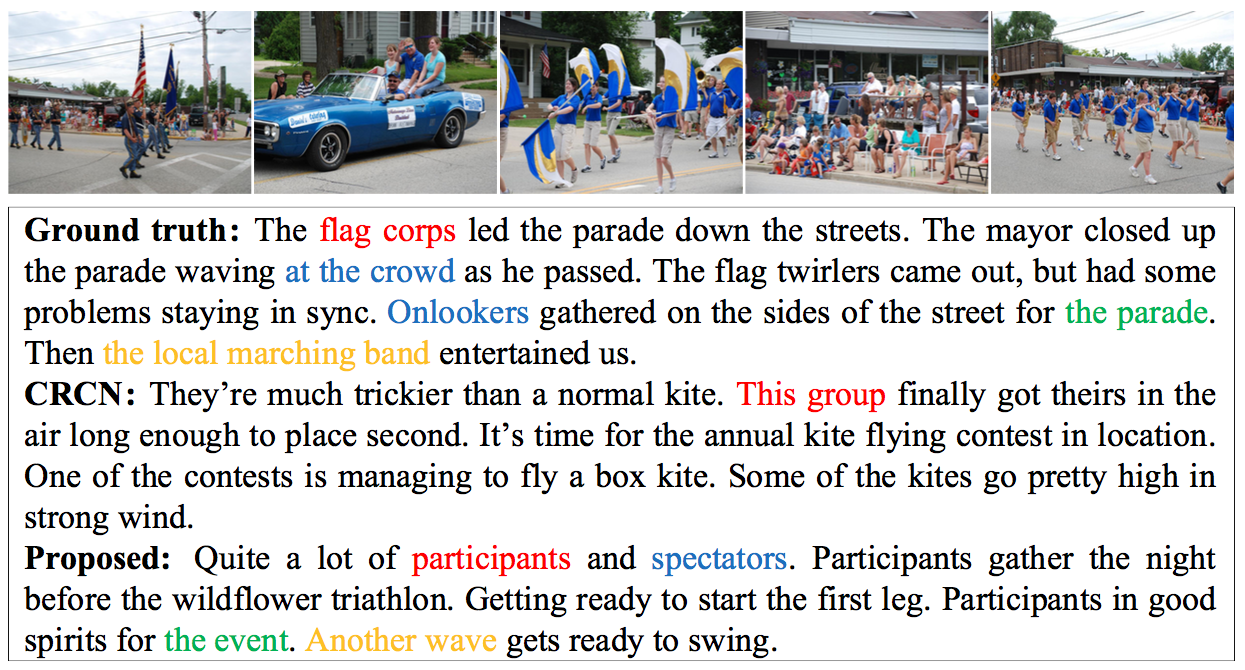
\includegraphics[width=0.5\textwidth]{BARNN}
\caption{Examples of visual storytelling result on SIND. Three stories are generated for each photo stream: story by GT, story by baseline CRCN and story by the proposed BARNN. The colored words indicate the semantic matches between the generation results with the GT \cite{liu2017let}}
\centering
\label{fg:BARNN}
\end{figure}

\begin{figure}[h]
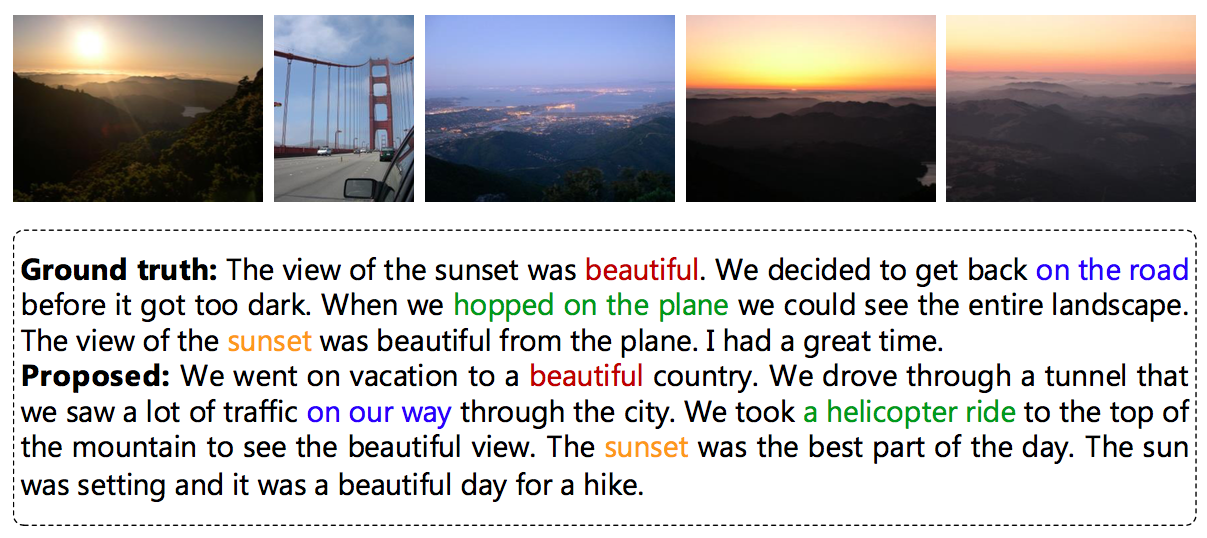
\includegraphics[width=0.5\textwidth]{Adversarial}
\caption{ Examples for narratives generated by the proposed model and stories from ground truth. The proposed is adversarial training model. The words in same colors
indicate the correct semantic matches between the generated narratives and those from ground truth \cite{show-reward-tell-automatic-generation-narrative-paragraph-photo-stream-adversarial-training}.}
\centering
\label{fg:Ad}
\end{figure}

\section{Discussion}
Compared with three different datasets, we can see from table \ref{tb:NYC}, table \ref{tb:Disney} and table \ref{tb:SIND}, BARNN model performs better than CRCN model in each dataset and each retrieval task. For example in table \ref{tb:SIND}, BARNN R@1 value is 24.07 where CRCN just is 9.87. The bigger recall top K value is, the better performance model has. It's the same as R@5 and R@10, the value 44.29 versus 28.74 and 53.06 versus 39.51. For median rank value, the less value is, the better performance the model has. Compared with BARNN median rank 9 with CRCN median rank 21, it confirms BARNN has better performance as well. 

The reason why BARNN performs better than CRCN is that BARNN using bidirectional RNN and also creates embedding space for images and narrative sentences, which could handle with large image variance. This advantage is CRCN lack of. The evidence is from table \ref{tb:SIND} methods BARNN-sGRU and BARNN-EMB compared with CRCN.  We can see that BARNN without sGRU or embedding space could perform better than CRCN as well and their value, for example R@1, without sGRU is 21.39 and without embedding space is 21.63, CRCN is just 9.87 and BARNN is 24.07. The number shows BRNN network performs quite better in this task than recurrent convolutional network. BRNN with sGRU and embedding space has micro-improvement than without.

For table \ref{tb:METEOR}, BARNN also has better quality of language generating in BLEU score and CIDEr value. Although these methods would be influenced by different language generating model, these values could partially confirm how generating sentence correlates with ground truth. See the figure \ref{fg:BARNN}, the colored words indicate the semantic matches between generation results with ground truth, and BARNN model has more similar semantic words mentioned in ground truth sentence compared with CRCN. For example the yellow word in ground truth \textit{local marching band}, in CRCN there is nothing related word to match it, but in BARNN \textit{Another wave} could be matched it.

Due to adversarial training model did not compare with CRCN and BARNN directly, so we just discuss their user study result in table \ref{tb:user}. This table shows that in both two criteria, relevance and story-style, BARNN performs better than CRCN, which to accord with our previous conclusion. However, Adversarial training model performs better than BARNN. In relevance criteria, adversarial training model's value is almost twice larger than BARNN's, but in story-style there is no quite large difference, which means relevance value could show how information density the generation sentence has and story-style value could show how languae model performance is. So it could be partially confirmed that Adversarial learning model has more powerful ability in image captioning than BARNN.

In my perspective of view, I think why adversarial model could perform better than the others is that introducing game theory would approach more to human brain operation. As rational agent, we learn different things from different games every moment. And learning is also a way like creating assumption and doing confirmation. This is quite similar as generative model and discriminative model.

At the end, we introduce threes different approaches in images story generating field and explain their basic principles. And then we discuss them difference and performance, explain the reason why they perform differently. We can see this images story generating task is solving step by step, from the initial CRCN approach to using BARNN, later stay at best performance Adversarial model till now. This interesting procedure of evolution also tells us when we use more artificial principles, we could be closer to the truth. 


\bibliography{bibliography}
\bibliographystyle{fss2017seminar}

\end{document}
